\documentclass[aspectratio=43]{beamer}
% Theme works only with a 4:3 aspect ratio
\usetheme{CSCS}

\usepackage{tikz}
\usepackage{pgfplots}
\usepackage{pgfplotstable}
\usetikzlibrary{pgfplots.groupplots,spy,patterns}
\usepackage{listings}
\usepackage{color}
\usepackage{tcolorbox}
\usepackage{anyfontsize}
\usepackage{xspace}
\usepackage{graphicx}

% define footer text
\newcommand{\footlinetext}{Introduction to GPUs in HPC}

% Select the image for the title page
\newcommand{\picturetitle}{cscs_images/image5.pdf}

% fonts for maths
\usefonttheme{professionalfonts}
\usefonttheme{serif}

% source code listing
\newcommand{\axpy}{{\ttfamily axpy}\xspace}

% set indent to a more reasonable level (so that itemize can be used in columns)
\setlength{\leftmargini}{20pt}

\DeclareTextFontCommand{\emph}{\bfseries\color{blue!70!black}}

% Please use the predifined colors:
% cscsred, cscsgrey, cscsgreen, cscsblue, cscsbrown, cscspurple, cscsyellow, cscsblack, cscswhite

\author{Ben Cumming, CSCS}
\title{Writing GPU Kernels}
\subtitle{}
\date{\today}

\begin{document}

% TITLE SLIDE
\cscstitle

% CHAPTER SLIDE
\cscschapter{Going Parallel: Working Together}

%%%%%%%%%%%%%%%%%%%%%%%%%%%%%%%%%%%%%%%%%%%%
\begin{frame}[fragile]{}
%%%%%%%%%%%%%%%%%%%%%%%%%%%%%%%%%%%%%%%%%%%%
    \centering
    Most algorithms do not lend themselves to trivial parallelization

%----------------------------
    \begin{code}{reductions : e.g. dot product}
        \begin{lstlisting}[style=boxcudatiny]
int dot(int *x, int *y, int n){
  int sum = 0;
  for(auto i=0; i<n; ++i)
    sum += x[i]*y[i];
  return sum;
}
        \end{lstlisting}
    \end{code}
%----------------------------
\vspace{-7pt}
%----------------------------
        \begin{code}{scan : e.g. prefix sum}
            \begin{lstlisting}[style=boxcudatiny]
void prefix_sum(int *x, int n){
  for(auto i=1; i<n; ++i)
    x[i] += x[i-1];
}
        \end{lstlisting}
    \end{code}
%----------------------------
\vspace{-7pt}
%----------------------------
    \begin{code}{fusing pipelined stencil loops : e.g. apply blur kernel twice}
        \begin{lstlisting}[style=boxcudatiny]
void twice_blur(float *in, float *out, int n){
  float buff[n];
  for(auto i=1; i<n-1; ++i)
    buff[i] = 0.25f*(in[i-1]+in[i+1]+2.f*in[i]);
  for(auto i=2; i<n-2; ++i)
    out[i] = 0.25f*(buff[i-1]+buff[i+1]+2.f*buff[i]);
}
        \end{lstlisting}
    \end{code}

\end{frame}

%%%%%%%%%%%%%%%%%%%%%%%%%%%%%%%%%%%%%%%%%%%%
\begin{frame}[fragile]{Block Level Synchronization}
%%%%%%%%%%%%%%%%%%%%%%%%%%%%%%%%%%%%%%%%%%%%
    \begin{columns}[T]
        \begin{column}{0.3\textwidth}
            \centering
            \includegraphics[width=\textwidth]{./images/smx.pdf}

            The P100 SMX has 64 KB of shared memory
        \end{column}

        \begin{column}{0.7\textwidth}
            CUDA provides mechanisms for \emph{cooperation between threads in a thread block}.
            \begin{itemize}
                \item All threads in a block run on the same SMX
                \item Resources for synchronization are at SMX level
                \item No synchronization between threads in different blocks
            \end{itemize}
            CUDA also supports global \emph{atomic operations} for coordination between threads
            \begin{itemize}
                \item We will cover this later\dots
            \end{itemize}
        \end{column}
    \end{columns}

\end{frame}

%%%%%%%%%%%%%%%%%%%%%%%%%%%%%%%%%%%%%%%%%%%%
\begin{frame}[fragile]{Block Level Synchronization}
%%%%%%%%%%%%%%%%%%%%%%%%%%%%%%%%%%%%%%%%%%%%
        Cooperation between threads requires sharing of data
        \begin{itemize}
            \item All threads in a block can share data using \emph{shared memory}.
            \item Shared memory is \emph{not visible} to threads in other thread blocks.
            \item All threads in a block are on the same SMX.
            \item There is 64 KB of shared memory on each SMX
            \begin{itemize}
                \item one thread block can allocate 64 KB for itself
                \item two thread blocks can allocate 32 KB each\dots
                \item \dots shared memory per thread block is a constraint on how many thread blocks can run simultaneously on an SMX.
            \end{itemize}
        \end{itemize}

\end{frame}

%%%%%%%%%%%%%%%%%%%%%%%%%%%%%%%%%%%%%%%%%%%%
\begin{frame}[fragile]{1D blur kernel}
%%%%%%%%%%%%%%%%%%%%%%%%%%%%%%%%%%%%%%%%%%%%
    A simple intensity preserving filter:
    \centering $\text{out}_i \leftarrow 0.25\times(\text{in}_{i-1}+2\times\text{in}_i+\text{in}_{i+1})$
    \begin{itemize}
        \item Each output value is a linear combination of neighbours in input array
        \item First we look at naive implementation
    \end{itemize}

    \begin{code}{Host implementation of blur kernel}
        \begin{lstlisting}[style=boxcudatiny]
void blur(double *in, double *out, int n){
  float buff[n];
  for(auto i=1; i<n-1; ++i)
    out[i] = 0.25*(in[i-1] + 2*in[i] + in[i+1]);
}
        \end{lstlisting}
    \end{code}

\end{frame}

%%%%%%%%%%%%%%%%%%%%%%%%%%%%%%%%%%%%%%%%%%%%
\begin{frame}[fragile]{1D blur kernel on GPU}
%%%%%%%%%%%%%%%%%%%%%%%%%%%%%%%%%%%%%%%%%%%%
    \begin{center}
        Our first CUDA implementation of the blur kernel has each thread load the three values required to form its output
    \end{center}
    \begin{code}{First implementation of blur kernel}
        \begin{lstlisting}[style=boxcudatiny]
__global__ void
blur(const double *in, double* out, int n) {
  int i = threadIdx.x + 1; // assume one thread block

  if(i<n-1) {
    out[i] = 0.25*(in[i-1] + 2*in[i] + in[i+1]);
  }
}
        \end{lstlisting}
    \end{code}

\end{frame}

%%%%%%%%%%%%%%%%%%%%%%%%%%%%%%%%%%%%%%%%%%%%
\begin{frame}[fragile]{}
%%%%%%%%%%%%%%%%%%%%%%%%%%%%%%%%%%%%%%%%%%%%
    \centering
    Each thread has to load 3 values from global memory to calculate its output \\
    \includegraphics[width=0.8\textwidth]{./images/blur_point_gather.pdf} \\
    Alternatively, each value in the input array has to be loaded 3 times \\
    \includegraphics[width=0.8\textwidth]{./images/blur_point_scatter.pdf} \\
\end{frame}

%%%%%%%%%%%%%%%%%%%%%%%%%%%%%%%%%%%%%%%%%%%%
\begin{frame}[fragile]{}
%%%%%%%%%%%%%%%%%%%%%%%%%%%%%%%%%%%%%%%%%%%%
    To take advantage of shared memory the kernel is split into two stages:
    \begin{enumerate}
        \item Load \lst{in[i]} into shared memory \lst{buffer[i]}.
        \begin{itemize}
            \item One thread has to load \lst{in[0]} \& \lst{in[n]}.
        \end{itemize}
        \item Use values \lst{buffer[i-1:i+1]} to compute kernel.
    \end{enumerate}

    \begin{center}
        \includegraphics[width=0.8\textwidth]{./images/blur_point_shared.pdf}
    \end{center}
\end{frame}

%%%%%%%%%%%%%%%%%%%%%%%%%%%%%%%%%%%%%%%%%%%%
\begin{frame}[fragile]{}
%%%%%%%%%%%%%%%%%%%%%%%%%%%%%%%%%%%%%%%%%%%%
    \begin{code}{Blur kernel with shared memory}
        \begin{lstlisting}[style=boxcudatiny]
__global__
void blur_shared_block(double *in, double* out, int n) {
    extern __shared__ double buffer[];

    auto i = threadIdx.x + 1;

    if(i<n-1) {
        // load shared memory
        buffer[i] = in[i];
        if(i==1) {
            buffer[0] = in[0];
            buffer[n-1] = in[n-1];
        }

        __syncthreads();

        out[i] = 0.25*(buffer[i-1] + 2.0*buffer[i] + buffer[i+1]);
    }
}
        \end{lstlisting}
    \end{code}

\end{frame}

%%%%%%%%%%%%%%%%%%%%%%%%%%%%%%%%%%%%%%%%%%%%
\begin{frame}[fragile]{Synchronizing threads}
%%%%%%%%%%%%%%%%%%%%%%%%%%%%%%%%%%%%%%%%%%%%
    The built-in CUDA function \lst{__syncthreads()} creates a barrier, where all threads in a thread block synchronize.
    \begin{itemize}
        \item Threads wait for all threads in thread block to finish loading shared memory buffer.
        \item Thread $i$ needs to wait for threads $i-1$ and $i+1$ to load values into \lst{buffer}.
        \item Synchronization required to avoid race conditions.
        \begin{itemize}
            \item Threads have to wait for other threads to fill \lst{buffer}.
        \end{itemize}
    \end{itemize}
\end{frame}

%%%%%%%%%%%%%%%%%%%%%%%%%%%%%%%%%%%%%%%%%%%%
\begin{frame}[fragile]{Declaring shared memory}
%%%%%%%%%%%%%%%%%%%%%%%%%%%%%%%%%%%%%%%%%%%%
    There are two ways to declare shared memory allocations.

    \begin{info}{Dynamic allocation}
        When the memory is determined at run time:
        \centering \lst{extern __shared__ double buffer[];}
        \begin{itemize}
            \item Note the \lst{extern} keyword.
            \item The size of memory to be allocated is specified when the kernel is launched.
        \end{itemize}
    \end{info}

    \begin{info}{Static allocation}
        When the amount of memory is known at compile time:
        \centering \lst{__shared__ double buffer[128];}
        \begin{itemize}
            \item Here there are 128 double-precision values (1024 bytes) of memory shared by all threads.
        \end{itemize}
    \end{info}

\end{frame}

%%%%%%%%%%%%%%%%%%%%%%%%%%%%%%%%%%%%%%%%%%%%
\begin{frame}[fragile]{Launching with static shared memory}
%%%%%%%%%%%%%%%%%%%%%%%%%%%%%%%%%%%%%%%%%%%%
    The amount of shared memory should be sufficient for the number of threads.

    \begin{code}{Using compile time bounds}
        \begin{lstlisting}[style=boxcudatiny]
template <int THREADS>
__global__
void kernel(...) {
  __shared__ double buffer[THREADS];

  // ... THREADS must equal blockDim.x
}

// launch kernel with threads per block as a template parameter
kernel<128>@<<<@num_blocks, 128@>>>@(...);
        \end{lstlisting}
    \end{code}
\end{frame}

%%%%%%%%%%%%%%%%%%%%%%%%%%%%%%%%%%%%%%%%%%%%
\begin{frame}[fragile]{Launching with static shared memory}
%%%%%%%%%%%%%%%%%%%%%%%%%%%%%%%%%%%%%%%%%%%%
    It is possible to allocate multiple variables as shared memory.
    \begin{itemize}
        \item   If the shared memory is used separately, you can use a union to ``overlap'' the storage.
        \item   Shared memory is a limited resource.
    \end{itemize}

    \begin{columns}[T]
        \begin{column}{0.48\textwidth}
            \begin{code}{separate storage}
                \begin{lstlisting}[style=boxcudatiny]
__global__
void kernel1() {
  // 1536 bytes
  __shared__ int X[128];
  __shared__ double Y[128];

  // OK
  X[i] = (int)Y[i];
}
                 \end{lstlisting}
            \end{code}
        \end{column}

        \begin{column}{0.48\textwidth}
            \begin{code}{overlapping storage}
                \begin{lstlisting}[style=boxcudatiny]
__global__
void kernel2(int n) {
  // 1024 bytes
  __shared__ union {
    int X[128];
    double Y[128];
  } buf;

  // not OK
  buf.X[i] = (int)buf.Y[i];
}
                \end{lstlisting}
            \end{code}
        \end{column}
    \end{columns}
\end{frame}

%%%%%%%%%%%%%%%%%%%%%%%%%%%%%%%%%%%%%%%%%%%%
\begin{frame}[fragile]{Finding resource usage of kernels}
%%%%%%%%%%%%%%%%%%%%%%%%%%%%%%%%%%%%%%%%%%%%
    The nvcc flag \lstterm{--resource-usage} will print the resources used by each kernel during compilation:
    \begin{itemize}
        \item shared memory
        \item constant memory
        \item registers
    \end{itemize}

    \begin{terminal}{using the \lstterm{--resource-usage} on kernels in previous slide}
    \begin{lstlisting}[style=terminal]
> nvcc --resource-usage -arch=sm_60 shared.cu 
ptxas info  : 0 bytes gmem
ptxas info  : Compiling entry function '_Z7kernel2i' for
ptxas info  : Function properties for _Z7kernel2i
0 bytes stack frame, 0 bytes spill stores, 0 bytes spill loads
ptxas info  : Used 6 registers, 1024 bytes smem, 324 bytes cmem[0]
ptxas info  : Compiling entry function '_Z7kernel1v' for
ptxas info  : Function properties for _Z7kernel1v
0 bytes stack frame, 0 bytes spill stores, 0 bytes spill loads
ptxas info  : Used 6 registers, 1536 bytes smem, 320 bytes cmem[0]
> c++filt _Z7kernel2i
kernel2(int)
    \end{lstlisting}
    \end{terminal}
    \emph{Note}: the kernel names have been mangled (use \lstterm{c++filt}.)

\end{frame}



%%%%%%%%%%%%%%%%%%%%%%%%%%%%%%%%%%%%%%%%%%%%
\begin{frame}[fragile]{Launching with dynamic shared memory}
%%%%%%%%%%%%%%%%%%%%%%%%%%%%%%%%%%%%%%%%%%%%
        An additional parameter is added to the launch syntax
        \\
        \centering \lst{blur``<<<``grid_dim, block_dim, shared_size``>>>``(...);}
        \begin{itemize}
            \item \lst{shared_size} is the shared memory \emph{in bytes} to be allocated \emph{per thread block}
        \end{itemize}

    \begin{code}{Launch blur kernel with shared memory}
        \begin{lstlisting}[style=boxcudatiny]
__global__
void blur_shared(double *in, double* out, int n) {
  extern __shared__ double buffer[];

  int i = threadIdx.x + 1;
  // ...
}

// in main()
auto block_dim = n-2;
auto size_in_bytes = n*sizeof(double);

blur_shared@<<<@1, block_dim, size_in_bytes@>>>@(x0, x1, n);
        \end{lstlisting}
    \end{code}

\end{frame}

%%%%%%%%%%%%%%%%%%%%%%%%%%%%%%%%%%%%%%%%%%%%
\begin{frame}[fragile]{}
%%%%%%%%%%%%%%%%%%%%%%%%%%%%%%%%%%%%%%%%%%%%
        A version of the blur kernel for arbitrarily large $n$ is provided in \lst{blur.cu} in the example code. The implementation is a bit awkward:
        \begin{itemize}
            \item  the \lst{in} and \lst{out} arrays use global indexes
            \item  the shared memory uses thread block local indexes
        \end{itemize}

    \begin{info}{Is it worth it?}
        \begin{itemize}
            \item on Keplar this optimization was worth $\approx$10\%.
            \item on P100 there is no speedup (I think due to improved read only L1 caching on P100)
        \end{itemize}
        The small performance improvement on Keplar was worth it if this was a key kernel in your application\dots
    \end{info}

\end{frame}

%%%%%%%%%%%%%%%%%%%%%%%%%%%%%%%%%%%%%%%%%%%%
\begin{frame}[fragile]{}
%%%%%%%%%%%%%%%%%%%%%%%%%%%%%%%%%%%%%%%%%%%%
    \begin{info}{Buffering}
        A pipelined workflow uses the output of one ``kernel'' as the input of another
        \begin{itemize}
            \item On the CPU these can be optimized by keeping the intermediate result in cache for the second kernel.
        \end{itemize}
        e.g. two stencils, one applied to the output of the first.
    \end{info}

    \begin{code}{Double blur: naive OpenMP}
        \begin{lstlisting}[style=boxcudatiny]
void blur_twice(const double* in , double* out , int n) {
  static double* buffer = malloc_host<double>(n);

  @#pragma omp parallel for@
  for(auto i=1; i<n-1; ++i) {
    buffer[i] = 0.25*( in[i-1] + 2.0*in[i] + in[i+1]);
  }
  @#pragma omp parallel for@
  for(auto i=2; i<n-2; ++i) {
    out[i] = 0.25*( buffer[i-1] + 2.0*buffer[i] + buffer[i+1]);
  }
}
        \end{lstlisting}
    \end{code}

\end{frame}

%%%%%%%%%%%%%%%%%%%%%%%%%%%%%%%%%%%%%%%%%%%%
\begin{frame}[fragile]{}
%%%%%%%%%%%%%%%%%%%%%%%%%%%%%%%%%%%%%%%%%%%%
    %For a host implementation break work into blocks, to keep intermediate results in \lst{buffer} in cache.
    \begin{code}{Double blur: OpenMP with blocking for cache}
        \begin{lstlisting}[style=boxcudatiny]
void blur_twice(const double* in , double* out , int n) {
  auto const block_size = std::min(512, n-4);
  auto const num_blocks = (n-4)/block_size;
  static double* buffer = malloc_host<double>((block_size+4)*omp_get_max_threads());

  auto blur = [] (int pos, const double* u) {
    return 0.25*( u[pos-1] + 2.0*u[pos] + u[pos+1]);
  };

  @#pragma omp parallel for@
  for(auto b=0; b<num_blocks; ++b) {
    auto tid = omp_get_thread_num();
    auto first = 2 + b*block_size;
    auto last = first + block_size;

    auto buff = buffer + tid*(block_size+4);
    for(auto i=first-1, j=1; i<(last+1); ++i, ++j) {
      buff[j] = blur(i, in);
    }
    for(auto i=first, j=2;   i<last;   ++i, ++j) {
      out[i] = blur(j, buff);
    }
  }
}
        \end{lstlisting}
    \end{code}
\end{frame}

%%%%%%%%%%%%%%%%%%%%%%%%%%%%%%%%%%%%%%%%%%%%
\begin{frame}[fragile]{}
%%%%%%%%%%%%%%%%%%%%%%%%%%%%%%%%%%%%%%%%%%%%
    \begin{info}{Buffering with shared memory}
        Shared memory is important for caching intermediate results used in pipelined operations.
        \begin{itemize}
            \item Shared memory is an order of magnitude faster than global DRAM.
            \item By \emph{fusing} pipelined operations in one kernel, intermediate results can be stored in shared memory.
            \item Similar to blocking and tiling for cache on the CPU.
        \end{itemize}
    \end{info}

\end{frame}


%%%%%%%%%%%%%%%%%%%%%%%%%%%%%%%%%%%%%%%%%%%%
\begin{frame}[fragile]{}
%%%%%%%%%%%%%%%%%%%%%%%%%%%%%%%%%%%%%%%%%%%%
    \begin{code}{Double blur: CUDA with shared memory}
        \begin{lstlisting}[style=boxcudatiny]
__global__ void blur_twice(const double *in, double* out, int n) {
  extern __shared__ double buffer[];

  auto block_start = blockDim.x * blockIdx.x;
  auto block_end   = block_start + blockDim.x;
  auto lid = threadIdx.x + 2;
  auto gid = lid + block_start;

  auto blur = [] (int pos, double const* field) {
    return 0.25*(field[pos-1] + 2.0*field[pos] + field[pos+1]);
  };

  if(gid<n-2) {
    buffer[li] = blur(gi, in);
    if(threadIdx.x==0) {
        buffer[1]            = blur(block_start+1, in);
        buffer[blockDim.x+2] = blur(block_end+2, in);
    }

    __syncthreads();

    out[gi] = blur(li, buffer);
  }
}
        \end{lstlisting}
    \end{code}
\end{frame}

%%%%%%%%%%%%%%%%%%%%%%%%%%%%%%%%%%%%%%%%%%%%
\begin{frame}[fragile]{}
%%%%%%%%%%%%%%%%%%%%%%%%%%%%%%%%%%%%%%%%%%%%
    \begin{info}{Fused loop results}
        The OpenMP cache-aware version was harder to implement than the shared-memory CUDA version:
        \begin{itemize}
            \item CUDA seems harder because we have to think and write in parallel from the start.
        \end{itemize}
        Both implementations benefit significantly from optimizations for fast on chip memory.
    \end{info}
    \begin{columns}[T]
        \begin{column}{0.5\textwidth}
            \centering
            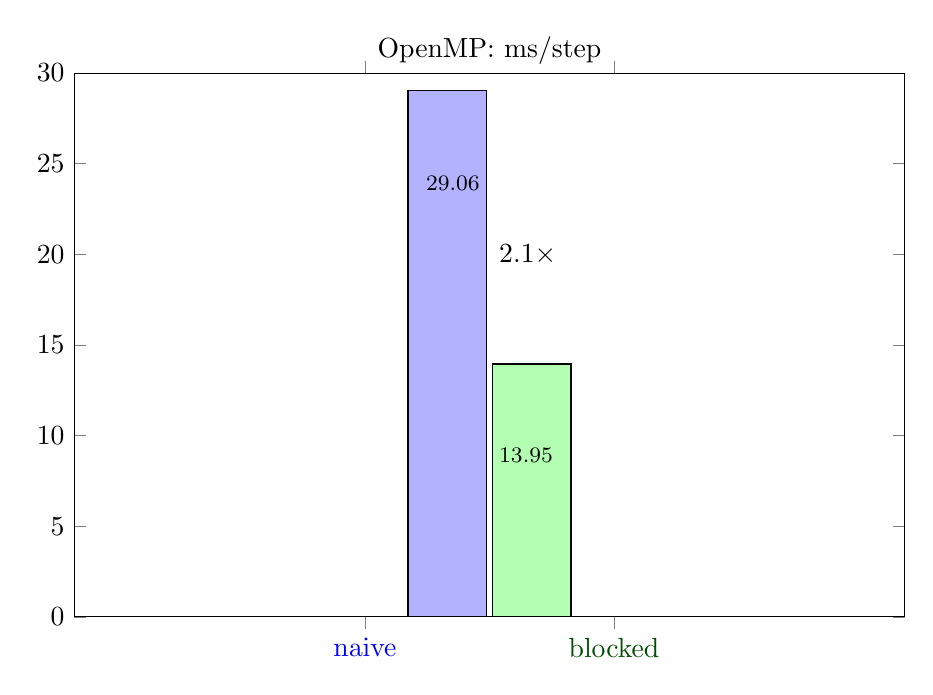
\begin{tikzpicture}
                \begin{axis}[
                    ybar,
                    height=0.7\textwidth,
                    width=\textwidth,
                    ymin=0,
                    ymax=30,
                    %ticks=none,
                    ytick={0,5,10,15,20,25,30},
                    title={OpenMP: ms/step},
                    title style={yshift=-1.5ex},
                    xtick={0.94, 1.06},
                    xticklabels={\color{blue}{naive}, \color{green!30!black}{blocked}}
                ]
                \addplot
                    [draw=black, fill=blue!30, bar width=1cm]
                    coordinates {(1,29.06)};
                \addplot
                    [draw=black, fill=green!30, bar width=1cm]
                    coordinates {(1,13.95)};
                \node[right] at (axis cs:1,20) {2.1$\times$};
                \node[above left] at (axis cs:1,23) {\footnotesize29.06};
                \node[above right] at (axis cs:1,8) {\footnotesize13.95};
                %\legend{\tiny na\"ive, \tiny optimized};
                \end{axis}
            \end{tikzpicture}
        \end{column}

        \begin{column}{0.5\textwidth}
            \centering
            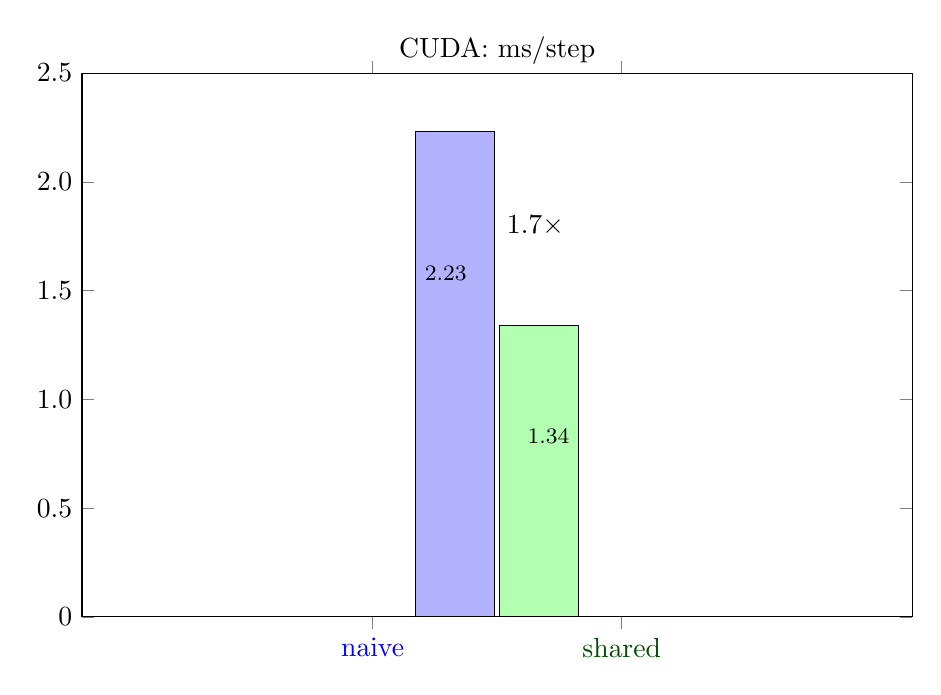
\begin{tikzpicture}
                \begin{axis}[
                    ybar,
                    height=0.7\textwidth,
                    width=\textwidth,
                    ymin=0,ymax=2.5,
                    %ticks=none,
                    ytick={0,0.5,1,1.5,2,2.5},
                    yticklabels={0,0.5,1.0,1.5,2.0,2.5},
                    title={CUDA: ms/step},
                    title style={yshift=-1.5ex},
                    xtick={0.94, 1.06},
                    xticklabels={\color{blue}{naive}, \color{green!30!black}{shared}}
                ]

                \addplot
                   [draw=black, fill=blue!30, bar width=1cm]
                    coordinates {(1,2.23)};
                \addplot
                   [draw=black, fill=green!30, bar width=1cm]
                    coordinates {(1,1.34)};
                \node[right] at (axis cs:1,1.8) {1.7$\times$};
                \node[above left] at (axis cs:0.99,1.5) {\footnotesize2.23};
                \node[above right] at (axis cs:1.01,0.75) {\footnotesize1.34};
                %\legend{\tiny na\"ive, \tiny optimized};
                \end{axis}
            \end{tikzpicture}
        \end{column}
    \end{columns}
    {\footnotesize OpenMP results with 18-core Broadwell CPU; CUDA with P100 GPU; $n=33,554,432$}
\end{frame}

%%%%%%%%%%%%%%%%%%%%%%%%%%%%%%%%%%%%%%%%%%%%
\begin{frame}[fragile]{}
%%%%%%%%%%%%%%%%%%%%%%%%%%%%%%%%%%%%%%%%%%%%
    \begin{info}{CPU : optimizing for on-chip memory}
        \begin{itemize}
            \item let hardware prefetcher automatically manage cache
            \item choose block/tile sizes so that intermediate data will fit in a target cache (L1, L2 or L3)
        \end{itemize}
    \end{info}
    \begin{info}{GPU : optimizing for on-chip memory}
        \begin{itemize}
            \item manage shared memory manually
            \begin{itemize}
                \item more control
                \item hardware-specific
            \end{itemize}
            \item choose thread block sizes so that intermediate data will fit into shared memory on an SMX
        \end{itemize}
    \end{info}

\end{frame}

%%%%%%%%%%%%%%%%%%%%%%%%%%%%%%%%%%%%%%%%%%%%
\begin{frame}[fragile]{Exercise: Shared Memory}
%%%%%%%%%%%%%%%%%%%%%%%%%%%%%%%%%%%%%%%%%%%%
    \begin{itemize}
        \item Finish the \lstterm{shared/string_reverse.cu} example. Assume $n\leq1024$.
        \begin{itemize}
            \item With or without shared memory.
            \item \emph{Extra}: without any synchronization.
        \end{itemize}
        \item Implement a dot product in CUDA in \lstterm{shared/dot.cu}.
        \begin{itemize}
            \item The host version has been implemented as \lst{dot_host()}
            \item Assume $n\leq1024$.
            \item \emph{Extra}: how would you extend it to work for arbitrary $n>1024$ and $n$ threads?
        \end{itemize}
    \end{itemize}

    \centering \includegraphics[width=0.5\textwidth]{./images/reduction.pdf}

\end{frame}

%%%%%%%%%%%%%%%%%%%%%%%%%%%%%%%%%%%%%%%%%%%%
\begin{frame}[fragile]{Communication}
%%%%%%%%%%%%%%%%%%%%%%%%%%%%%%%%%%%%%%%%%%%%
    Communication in a GPU code occurs at different levels:
    \begin{itemize}
        \item Between threads in a warp;
        \item Between threads in thread block;
        \item Between threads in grid;
        \item Between threads in different grids.
    \end{itemize}
    Involves reading and writing shared resources:
    \begin{itemize}
        \item Synchronization required if more than one thread wants to modify (write) a shared resource.
    \end{itemize}
\end{frame}

%%%%%%%%%%%%%%%%%%%%%%%%%%%%%%%%%%%%%%%%%%%%
\begin{frame}[fragile]{Race conditions}
%%%%%%%%%%%%%%%%%%%%%%%%%%%%%%%%%%%%%%%%%%%%
        A race condition can occur when more than one thread attempts to access the same memory location concurrently and at least one access is a write.

\begin{columns}[T]
    \begin{column}{0.45\textwidth}
    \begin{code}{}
        \begin{lstlisting}[style=boxcudatiny]
__global__
void race(int* x) {
  ++x[0]
}

int main(void) {
  int* x =
    malloc_managed<int>(1);
  race@<<<@1, 2@>>>@(x);
  cudaDeviceSynchronize();
  // what value is in x[0]?
}
        \end{lstlisting}
    \end{code}
    \end{column}
    \begin{column}[T]{0.55\textwidth}
        \begin{center}\scriptsize
            \vspace{-0.7cm}
            \textsc{No Race} \hspace{1.5cm} \textsc{Race} \\
            \vspace{0.1cm}
        \begin{tabular}[]{|ccc|}
            \hline
             t0 &  t1 &  $x$ \\
            \hline
              R   &      &  0\\
              I   &      &  0\\
              W   &      &  1\\
                  & R    &  1\\
                  & I    &  1\\
                  & W    &  2\\
            \hline
        \end{tabular}
        \hspace{0.5cm}
        \begin{tabular}[]{|ccc|}
            \hline
             t0 &  t1 &  $x$ \\
            \hline
              R   &      &  0\\
                  &  R   &  0\\
              I   &      &  0\\
              W   &      &  1\\
                  &  I   &  1\\
                  &  W   &  1\\
            \hline
        \end{tabular}
        \end{center}
        \begin{center}
            \scriptsize
            Example where two threads \lstterm{t0} and \lstterm{t1} both increment $x$ in memory. The threads use: read (R); write (W); and increment (I).
        \end{center}
    \end{column}
\end{columns}

    \begin{itemize}
        \item Race conditions produce strange and unpredictable results.
        \item Synchronization is required to avoid race conditions.
    \end{itemize}
\end{frame}


%%%%%%%%%%%%%%%%%%%%%%%%%%%%%%%%%%%%%%%%%%%%
\begin{frame}[fragile]{Synchronization within a block}
%%%%%%%%%%%%%%%%%%%%%%%%%%%%%%%%%%%%%%%%%%%%
    Threads in the same thread block can use \lst{__syncthreads()} to synchronize on access to shared memory and global memory

    \begin{code}{synchronization on global memory}
        \begin{lstlisting}[style=boxcudatiny]
__global__
void update(int* x, int* y) {
  int i = threadIdx.x;
  if (i == 0) x[0] = 1;
  __syncthreads();
  if (i == 1) y[0] = x[0];
}

int main(void) {
  int* x = malloc_managed<int>(1);
  int* y = malloc_managed<int>(1);
  update@<<<@1,2@>>>@(x, y);
  cudaDeviceSynchronize();
  // both x[0] and y[0] equal 1
}
        \end{lstlisting}
    \end{code}

    \emph{Note}: All threads in a block must reach the \lst{__syncthreads()}
    \begin{itemize}
        \item otherwise strange things happen!
    \end{itemize}
\end{frame}

%%%%%%%%%%%%%%%%%%%%%%%%%%%%%%%%%%%%%%%%%%%%
\begin{frame}[fragile]{Atomic Operations: motivation}
%%%%%%%%%%%%%%%%%%%%%%%%%%%%%%%%%%%%%%%%%%%%
    What is the output of the following code?
    \begin{code}{}
        \begin{lstlisting}[style=boxcudatiny]
#include <cstdio>
#include <cstlib>
#include <cuda.h>
#include "util.hpp"

__global__ void count_zeros(int* x, int* count) {
  int i = threadIdx.x;
  if (x[i]==0) *count+=1;
}

int main(void) {
  int* x = malloc_managed<int>(1024);
  int* count = malloc_managed<int>(1);
  count = 0;
  for (int i=0; i<1024; ++i) x[i]=i%128;

  count_zeros@<<<@1, 1024@>>>@(x, count);
  cudaDeviceSynchronize();
  printf("result %d\n", *x); // expect 8

  cudaFree(x);
  return 0;
}
        \end{lstlisting}
    \end{code}

\end{frame}

%%%%%%%%%%%%%%%%%%%%%%%%%%%%%%%%%%%%%%%%%%%%
\begin{frame}[fragile]{Atomic Operations}
%%%%%%%%%%%%%%%%%%%%%%%%%%%%%%%%%%%%%%%%%%%%
    An \emph{atomic memory operation} is an uninterruptable read-modify-write memory operation:
    \begin{itemize}
        \item Serializes contentious updates from multiple threads;
        \item The order in which concurrent atomic updates are performed is not defined;
        \item However none of the atomic updates will be lost.
    \end{itemize}
    \vspace{-0.3cm}
    \begin{columns}[T]
        \begin{column}{0.48\textwidth}
            \begin{code}{race}
                \begin{lstlisting}[style=boxcudatiny]
__global__ void inc(int* x) {
  *x += 1;
}
                 \end{lstlisting}
            \end{code}
        \end{column}

        \begin{column}{0.48\textwidth}
            \begin{code}{no race}
                \begin{lstlisting}[style=boxcudatiny]
__global__ void inc(int* x) {
  atomicAdd(x, 1);
}
                \end{lstlisting}
            \end{code}
        \end{column}
    \end{columns}

    \begin{code}{}
        \begin{lstlisting}[style=boxcudatiny]
// pseudo-code implementation of atomicAdd
__device__ int atomicAdd(int *p, int v) {
  int old;
  exclusive_single_thread {
    old = *p; // Load from memory
    *p = old + v; // Store after adding v
  }
  return old; // return original value before modification
}
        \end{lstlisting}
    \end{code}

\end{frame}

%%%%%%%%%%%%%%%%%%%%%%%%%%%%%%%%%%%%%%%%%%%%
\begin{frame}[fragile]{Atomic Functions}
%%%%%%%%%%%%%%%%%%%%%%%%%%%%%%%%%%%%%%%%%%%%
    CUDA has a range of atomic funtions, including:
    \begin{itemize}
        \item \emph{Arithmetic}:
            \lstterm{atomicAdd()}, \lstterm{atomicSub()}, \lstterm{atomicMax()}, \lstterm{atomicMin()}, \lstterm{atomicCAS()}, \lstterm{atomicExch()}.
        \item \emph{Logical}: 
            \lstterm{atomicAnd()}, \lstterm{atomicOr()}, \lstterm{atomicXor()}.
    \end{itemize}
    These functions take both 32 and 64 bit arguments
    \begin{itemize}
        \item \lstterm{atomicAdd()} gained supported for \lstterm{double} in CUDA 8 with Pascal.
        \item see the \href{https://docs.nvidia.com/cuda/cuda-c-programming-guide/index.html#atomic-functions}{\textcolor{blue}{CUDA Programming Guide}} for specific details.
    \end{itemize}
\end{frame}

%%%%%%%%%%%%%%%%%%%%%%%%%%%%%%%%%%%%%%%%%%%%
\begin{frame}[fragile]{Atomic Performance}
%%%%%%%%%%%%%%%%%%%%%%%%%%%%%%%%%%%%%%%%%%%%
    Atomic operations are a blunt instrument:
    \begin{itemize}
        \item Even without contention, atomics are slower than normal accesses (loads, stores);
        \item Performance can degrade when many threads attempt atomic operations on few memory locations.
    \end{itemize}
    Try to avoid or minimise the number of atomic operations.
    \begin{itemize}
        \item Attempt to use shared memory and structure algorithms to avoid synchronization wherever possible.
        \item Try performing operation at warp level or block level.
        \item Use atomics for infrequent, sparse and/pr unpredictable global communication.
    \end{itemize}
\end{frame}

%%%%%%%%%%%%%%%%%%%%%%%%%%%%%%%%%%%%%%%%%%%%
\begin{frame}[fragile]{Exercises: Atomics}
%%%%%%%%%%%%%%%%%%%%%%%%%%%%%%%%%%%%%%%%%%%%
    \begin{itemize}
        \item What is \lstterm{shared/hist.cu} supposed to do?
        \begin{itemize}
            \item What is the output?
            \item Fix it to get the expected output.
        \end{itemize}
    \item Improve \lstterm{shared/dot.cu} to work for arbitrary $n$
    \end{itemize}
\end{frame}


%%%%%%%%%%%%%%%%%%%%%%%%%%%%%%%%%%%%%%%%%%%%
%\begin{frame}[fragile]{Warps}
%%%%%%%%%%%%%%%%%%%%%%%%%%%%%%%%%%%%%%%%%%%%
%    Threads blocks are partitioned into groups of threads called \emph{warps}
%    \begin{itemize}
%        \item \lst{auto warp_id = threadIdx.x\%warp_size;}
%        \item currently \lstterm{warp_size} is 32, however this might change.
%    \end{itemize}
%    An SMX schedules warps for execution
%    \begin{itemize}
%        \item no overhead for switching between warps
%        \item when a warp is selected to run, all threads in warp execute the same instruction.
%    \end{itemize}
%
%\end{frame}


\end{document}
